
%% bare_conf_compsoc.tex
%% V1.4b
%% 2015/08/26
%% by Michael Shell
%% See:
%% http://www.michaelshell.org/
%% for current contact information.
%%
%% This is a skeleton file demonstrating the use of IEEEtran.cls
%% (requires IEEEtran.cls version 1.8b or later) with an IEEE Computer
%% Society conference paper.
%%
%% Support sites:
%% http://www.michaelshell.org/tex/ieeetran/
%% http://www.ctan.org/pkg/ieeetran
%% and
%% http://www.ieee.org/

%%*************************************************************************
%% Legal Notice:
%% This code is offered as-is without any warranty either expressed or
%% implied; without even the implied warranty of MERCHANTABILITY or
%% FITNESS FOR A PARTICULAR PURPOSE! 
%% User assumes all risk.
%% In no event shall the IEEE or any contributor to this code be liable for
%% any damages or losses, including, but not limited to, incidental,
%% consequential, or any other damages, resulting from the use or misuse
%% of any information contained here.
%%
%% All comments are the opinions of their respective authors and are not
%% necessarily endorsed by the IEEE.
%%
%% This work is distributed under the LaTeX Project Public License (LPPL)
%% ( http://www.latex-project.org/ ) version 1.3, and may be freely used,
%% distributed and modified. A copy of the LPPL, version 1.3, is included
%% in the base LaTeX documentation of all distributions of LaTeX released
%% 2003/12/01 or later.
%% Retain all contribution notices and credits.
%% ** Modified files should be clearly indicated as such, including  **
%% ** renaming them and changing author support contact information. **
%%*************************************************************************


% *** Authors should verify (and, if needed, correct) their LaTeX system  ***
% *** with the testflow diagnostic prior to trusting their LaTeX platform ***
% *** with production work. The IEEE's font choices and paper sizes can   ***
% *** trigger bugs that do not appear when using other class files.       ***                          ***
% The testflow support page is at:
% http://www.michaelshell.org/tex/testflow/



\documentclass[conference,compsoc]{IEEEtran}
% Some/most Computer Society conferences require the compsoc mode option,
% but others may want the standard conference format.
%
% If IEEEtran.cls has not been installed into the LaTeX system files,
% manually specify the path to it like:
% \documentclass[conference,compsoc]{../sty/IEEEtran}





% Some very useful LaTeX packages include:
% (uncomment the ones you want to load)


% *** MISC UTILITY PACKAGES ***
%
%\usepackage{ifpdf}
% Heiko Oberdiek's ifpdf.sty is very useful if you need conditional
% compilation based on whether the output is pdf or dvi.
% usage:
% \ifpdf
%   % pdf code
% \else
%   % dvi code
% \fi
% The latest version of ifpdf.sty can be obtained from:
% http://www.ctan.org/pkg/ifpdf
% Also, note that IEEEtran.cls V1.7 and later provides a builtin
% \ifCLASSINFOpdf conditional that works the same way.
% When switching from latex to pdflatex and vice-versa, the compiler may
% have to be run twice to clear warning/error messages.

\newcommand\defeq{\stackrel{\mathclap{\tiny\mbox{def}}}{=}}
\DeclareMathAlphabet{\mathpzc}{OT1}{pzc}{m}{it}
\usepackage{mathtools}
\usepackage{amsthm,amssymb}
\usepackage{epstopdf}
\usepackage{epsfig}
%\usepackage[hidelinks]{hyperref}

\newtheorem{theorem}{Theorem}
\newtheorem{fact}{Fact}
\newtheorem{hypothesis}{Hypothesis}
\newtheorem{conjecture}{Conjecture}
\newtheorem{lemma}{Lemma}
\newtheorem{definition}{Definition}

\newcommand{\aj}    {\mbox{\it AJ}}
\newcommand{\bc}    {\mbox{\it BC}}
\newcommand{\bd}    {\mbox{\it BD}}
\newcommand{\br}    {\mbox{\it BR}}
\newcommand{\bt}    {\mbox{\it BT}}
\newcommand{\hb}    {\mbox{\it HB}}
\newcommand{\ih}    {\mbox{\it IH}}
\newcommand{\wc}    {\mbox{\it WC}}
\newcommand{\wcd}   {\mbox{\it WD}}
\newcommand{\wl}       {\mbox{\it WL}}
\newcommand{\wo}     {\mbox{\it WO}}
\renewcommand{\wr}  {\mbox{\it WR}}
\newcommand{\wt}    {\mbox{\it WT}}
\newcommand{\bu}    {\mbox{\it BU}}



% *** CITATION PACKAGES ***
%
\ifCLASSOPTIONcompsoc
  % IEEE Computer Society needs nocompress option
  % requires cite.sty v4.0 or later (November 2003)
  \usepackage[nocompress]{cite}
\else
  % normal IEEE
  \usepackage{cite}
\fi
% cite.sty was written by Donald Arseneau
% V1.6 and later of IEEEtran pre-defines the format of the cite.sty package
% \cite{} output to follow that of the IEEE. Loading the cite package will
% result in citation numbers being automatically sorted and properly
% "compressed/ranged". e.g., [1], [9], [2], [7], [5], [6] without using
% cite.sty will become [1], [2], [5]--[7], [9] using cite.sty. cite.sty's
% \cite will automatically add leading space, if needed. Use cite.sty's
% noadjust option (cite.sty V3.8 and later) if you want to turn this off
% such as if a citation ever needs to be enclosed in parenthesis.
% cite.sty is already installed on most LaTeX systems. Be sure and use
% version 5.0 (2009-03-20) and later if using hyperref.sty.
% The latest version can be obtained at:
% http://www.ctan.org/pkg/cite
% The documentation is contained in the cite.sty file itself.
%
% Note that some packages require special options to format as the Computer
% Society requires. In particular, Computer Society  papers do not use
% compressed citation ranges as is done in typical IEEE papers
% (e.g., [1]-[4]). Instead, they list every citation separately in order
% (e.g., [1], [2], [3], [4]). To get the latter we need to load the cite
% package with the nocompress option which is supported by cite.sty v4.0
% and later.





% *** GRAPHICS RELATED PACKAGES ***
%
\ifCLASSINFOpdf
  % \usepackage[pdftex]{graphicx}
  % declare the path(s) where your graphic files are
  % \graphicspath{{../pdf/}{../jpeg/}}
  % and their extensions so you won't have to specify these with
  % every instance of \includegraphics
  % \DeclareGraphicsExtensions{.pdf,.jpeg,.png}
\else
  % or other class option (dvipsone, dvipdf, if not using dvips). graphicx
  % will default to the driver specified in the system graphics.cfg if no
  % driver is specified.
  % \usepackage[dvips]{graphicx}
  % declare the path(s) where your graphic files are
  % \graphicspath{{../eps/}}
  % and their extensions so you won't have to specify these with
  % every instance of \includegraphics
  % \DeclareGraphicsExtensions{.eps}
\fi
% graphicx was written by David Carlisle and Sebastian Rahtz. It is
% required if you want graphics, photos, etc. graphicx.sty is already
% installed on most LaTeX systems. The latest version and documentation
% can be obtained at: 
% http://www.ctan.org/pkg/graphicx
% Another good source of documentation is "Using Imported Graphics in
% LaTeX2e" by Keith Reckdahl which can be found at:
% http://www.ctan.org/pkg/epslatex
%
% latex, and pdflatex in dvi mode, support graphics in encapsulated
% postscript (.eps) format. pdflatex in pdf mode supports graphics
% in .pdf, .jpeg, .png and .mps (metapost) formats. Users should ensure
% that all non-photo figures use a vector format (.eps, .pdf, .mps) and
% not a bitmapped formats (.jpeg, .png). The IEEE frowns on bitmapped formats
% which can result in "jaggedy"/blurry rendering of lines and letters as
% well as large increases in file sizes.
%
% You can find documentation about the pdfTeX application at:
% http://www.tug.org/applications/pdftex





% *** MATH PACKAGES ***
%
%\usepackage{amsmath}
% A popular package from the American Mathematical Society that provides
% many useful and powerful commands for dealing with mathematics.
%
% Note that the amsmath package sets \interdisplaylinepenalty to 10000
% thus preventing page breaks from occurring within multiline equations. Use:
%\interdisplaylinepenalty=2500
% after loading amsmath to restore such page breaks as IEEEtran.cls normally
% does. amsmath.sty is already installed on most LaTeX systems. The latest
% version and documentation can be obtained at:
% http://www.ctan.org/pkg/amsmath





% *** SPECIALIZED LIST PACKAGES ***
%
%\usepackage{algorithmic}
% algorithmic.sty was written by Peter Williams and Rogerio Brito.
% This package provides an algorithmic environment fo describing algorithms.
% You can use the algorithmic environment in-text or within a figure
% environment to provide for a floating algorithm. Do NOT use the algorithm
% floating environment provided by algorithm.sty (by the same authors) or
% algorithm2e.sty (by Christophe Fiorio) as the IEEE does not use dedicated
% algorithm float types and packages that provide these will not provide
% correct IEEE style captions. The latest version and documentation of
% algorithmic.sty can be obtained at:
% http://www.ctan.org/pkg/algorithms
% Also of interest may be the (relatively newer and more customizable)
% algorithmicx.sty package by Szasz Janos:
% http://www.ctan.org/pkg/algorithmicx




% *** ALIGNMENT PACKAGES ***
%
%\usepackage{array}
% Frank Mittelbach's and David Carlisle's array.sty patches and improves
% the standard LaTeX2e array and tabular environments to provide better
% appearance and additional user controls. As the default LaTeX2e table
% generation code is lacking to the point of almost being broken with
% respect to the quality of the end results, all users are strongly
% advised to use an enhanced (at the very least that provided by array.sty)
% set of table tools. array.sty is already installed on most systems. The
% latest version and documentation can be obtained at:
% http://www.ctan.org/pkg/array


% IEEEtran contains the IEEEeqnarray family of commands that can be used to
% generate multiline equations as well as matrices, tables, etc., of high
% quality.




% *** SUBFIGURE PACKAGES ***
%\ifCLASSOPTIONcompsoc
%  \usepackage[caption=false,font=footnotesize,labelfont=sf,textfont=sf]{subfig}
%\else
%  \usepackage[caption=false,font=footnotesize]{subfig}
%\fi
% subfig.sty, written by Steven Douglas Cochran, is the modern replacement
% for subfigure.sty, the latter of which is no longer maintained and is
% incompatible with some LaTeX packages including fixltx2e. However,
% subfig.sty requires and automatically loads Axel Sommerfeldt's caption.sty
% which will override IEEEtran.cls' handling of captions and this will result
% in non-IEEE style figure/table captions. To prevent this problem, be sure
% and invoke subfig.sty's "caption=false" package option (available since
% subfig.sty version 1.3, 2005/06/28) as this is will preserve IEEEtran.cls
% handling of captions.
% Note that the Computer Society format requires a sans serif font rather
% than the serif font used in traditional IEEE formatting and thus the need
% to invoke different subfig.sty package options depending on whether
% compsoc mode has been enabled.
%
% The latest version and documentation of subfig.sty can be obtained at:
% http://www.ctan.org/pkg/subfig




% *** FLOAT PACKAGES ***
%
%\usepackage{fixltx2e}
% fixltx2e, the successor to the earlier fix2col.sty, was written by
% Frank Mittelbach and David Carlisle. This package corrects a few problems
% in the LaTeX2e kernel, the most notable of which is that in current
% LaTeX2e releases, the ordering of single and double column floats is not
% guaranteed to be preserved. Thus, an unpatched LaTeX2e can allow a
% single column figure to be placed prior to an earlier double column
% figure.
% Be aware that LaTeX2e kernels dated 2015 and later have fixltx2e.sty's
% corrections already built into the system in which case a warning will
% be issued if an attempt is made to load fixltx2e.sty as it is no longer
% needed.
% The latest version and documentation can be found at:
% http://www.ctan.org/pkg/fixltx2e


%\usepackage{stfloats}
% stfloats.sty was written by Sigitas Tolusis. This package gives LaTeX2e
% the ability to do double column floats at the bottom of the page as well
% as the top. (e.g., "\begin{figure*}[!b]" is not normally possible in
% LaTeX2e). It also provides a command:
%\fnbelowfloat
% to enable the placement of footnotes below bottom floats (the standard
% LaTeX2e kernel puts them above bottom floats). This is an invasive package
% which rewrites many portions of the LaTeX2e float routines. It may not work
% with other packages that modify the LaTeX2e float routines. The latest
% version and documentation can be obtained at:
% http://www.ctan.org/pkg/stfloats
% Do not use the stfloats baselinefloat ability as the IEEE does not allow
% \baselineskip to stretch. Authors submitting work to the IEEE should note
% that the IEEE rarely uses double column equations and that authors should try
% to avoid such use. Do not be tempted to use the cuted.sty or midfloat.sty
% packages (also by Sigitas Tolusis) as the IEEE does not format its papers in
% such ways.
% Do not attempt to use stfloats with fixltx2e as they are incompatible.
% Instead, use Morten Hogholm'a dblfloatfix which combines the features
% of both fixltx2e and stfloats:
%
% \usepackage{dblfloatfix}
% The latest version can be found at:
% http://www.ctan.org/pkg/dblfloatfix




% *** PDF, URL AND HYPERLINK PACKAGES ***
%
%\usepackage{url}
% url.sty was written by Donald Arseneau. It provides better support for
% handling and breaking URLs. url.sty is already installed on most LaTeX
% systems. The latest version and documentation can be obtained at:
% http://www.ctan.org/pkg/url
% Basically, \url{my_url_here}.




% *** Do not adjust lengths that control margins, column widths, etc. ***
% *** Do not use packages that alter fonts (such as pslatex).         ***
% There should be no need to do such things with IEEEtran.cls V1.6 and later.
% (Unless specifically asked to do so by the journal or conference you plan
% to submit to, of course. )


% correct bad hyphenation here
\hyphenation{op-tical net-works semi-conduc-tor}


\begin{document}
%
% paper title
% Titles are generally capitalized except for words such as a, an, and, as,
% at, but, by, for, in, nor, of, on, or, the, to and up, which are usually
% not capitalized unless they are the first or last word of the title.
% Linebreaks \\ can be used within to get better formatting as desired.
% Do not put math or special symbols in the title.
\title{Towards best-case response times of real-time tasks \\
	under fixed-priority scheduling with preemption thresholds}


% author names and affiliations
% use a multiple column layout for up to three different
% affiliations
\author{\IEEEauthorblockN{H.J. Rivera Verduzco}
	\IEEEauthorblockA{Technische Universiteit Eindhoven (TU/e),\\
		Den Dolech 2, 5600 AZ Eindhoven,\\
		The Netherlands\\
		\textit{h.j.rivera.verduzco@student.tue.nl}}
	\and
	\IEEEauthorblockN{Reinder J. Bril}
	\IEEEauthorblockA{Technische Universiteit Eindhoven (TU/e),\\
		Den Dolech 2, 5600 AZ Eindhoven,\\
		The Netherlands\\
		\textit{r.j.bril@tue.nl}}}

% conference papers do not typically use \thanks and this command
% is locked out in conference mode. If really needed, such as for
% the acknowledgment of grants, issue a \IEEEoverridecommandlockouts
% after \documentclass

% for over three affiliations, or if they all won't fit within the width
% of the page (and note that there is less available width in this regard for
% compsoc conferences compared to traditional conferences), use this
% alternative format:
% 
%\author{\IEEEauthorblockN{Michael Shell\IEEEauthorrefmark{1},
%Homer Simpson\IEEEauthorrefmark{2},
%James Kirk\IEEEauthorrefmark{3}, 
%Montgomery Scott\IEEEauthorrefmark{3} and
%Eldon Tyrell\IEEEauthorrefmark{4}}
%\IEEEauthorblockA{\IEEEauthorrefmark{1}School of Electrical and Computer Engineering\\
%Georgia Institute of Technology,
%Atlanta, Georgia 30332--0250\\ Email: see http://www.michaelshell.org/contact.html}
%\IEEEauthorblockA{\IEEEauthorrefmark{2}Twentieth Century Fox, Springfield, USA\\
%Email: homer@thesimpsons.com}
%\IEEEauthorblockA{\IEEEauthorrefmark{3}Starfleet Academy, San Francisco, California 96678-2391\\
%Telephone: (800) 555--1212, Fax: (888) 555--1212}
%\IEEEauthorblockA{\IEEEauthorrefmark{4}Tyrell Inc., 123 Replicant Street, Los Angeles, California 90210--4321}}




% use for special paper notices
%\IEEEspecialpapernotice{(Invited Paper)}




% make the title area
\maketitle

% As a general rule, do not put math, special symbols or citations
% in the abstract
\begin{abstract}
Fixed-priority scheduling with preemption thresholds (FPTS) is supported by the AUTOSAR and OSEK standards as a scheduling policy. Since FPTS is a generalization of fixed-priority preemptive scheduling (FPPS) and fixed-priority non-preemptive scheduling (FPNS), it aims to improve schedulability. In this paper, we prove, as an intermediate step towards the exact best-case response time analysis for FPTS, that the best-case computation time of a non-preemptive task scheduled under FPTS or FPNS is a tight lower bound for its response time. In addition, we illustrate by means of an example that the best-case response time analysis for FPTS is most likely not a straight forward extension of the current best-case analysis for FPPS.
\end{abstract}

% no keywords



% For peer review papers, you can put extra information on the cover
% page as needed:
% \ifCLASSOPTIONpeerreview
% \begin{center} \bfseries EDICS Category: 3-BBND \end{center}
% \fi
%
% For peerreview papers, this IEEEtran command inserts a page break and
% creates the second title. It will be ignored for other modes.
\IEEEpeerreviewmaketitle



\section{Introduction}
Fixed-priority scheduling with preemption thresholds (FPTS) was first introduced in the ThreadX kernel \cite{TX} to limit the number of preemptions that a task may experience with the aim to improve schedulability and reduce preemption overheads compared to fixed-priority preemptive scheduling (FPPS). It is currently also supported by the automotive standards AUTOSAR and OSEK \iffalse\cite{AUT10}\cite{OSEK05} \fi[2, 3]. Although the worst-case response time analysis for FPTS has been studied extensively in the literature \iffalse\cite{WS99} \cite{R02} \cite{KRL05}\fi [4-6], little attention has been paid to its best-case counterpart.

FPTS is a generalization of FPPS and fixed-priority non-preemptive scheduling (FPNS). Therefore, it could be desirable to consider first the best-case response time analysis for FPPS and FPNS before investigating the corresponding analysis for FPTS. In particular, the best-case response time analysis for FPPS has been addressed in \cite{RS02} for constraint deadlines and in \cite{BLM13} for arbitrary deadlines. On the other hand, the best-case response time for FPNS has not been formally studied. 

FPNS is widely used in message-based protocols under a network environment. For example, the Controller Area Network (CAN) uses a priority based arbitration and non-preemptive scheduling for message transmission. Furthermore, special attention has been paid to the worst-case analysis for CAN in \cite{DBBL07}, and for FPNS in \cite{BLV09} to guarantee real-time requirements. However, when considering jitter induced by a network, it becomes relevant to study best-case response times next to worst-case response times of messages scheduled under FPNS.

In \cite{BV05}, a lower bound for the best-case response time under fixed-priority scheduling with deferred preemptions (FPDS) is presented. Since FPNS is a special case of FPDS, this analysis also applies for FPNS. In particular, this analysis gives the trivial result that the best-case computation time of a task is a lower bound for the best-case response time of such a task under FPNS. However, we would like to investigate whether this lower bound is tight for all cases.

The rest of this paper is organized as follows. Section 2 introduces the basic real-time scheduling model for FPTS as well as some related notions. The best-case response time for non-preemptive tasks is presented in Section 3. Section 4 introduces an example that shows that the best-case response time analysis for FPTS is most likely not a trivial extension of the current best-case analysis for FPPS. Finally, we conclude this paper in Section 5.

\section{Real-time scheduling model}
In this section, we present the real-time scheduling model for FPTS along with some related notions.

\subsection{Basic model for FPTS}
We assume a single processor and a set $\mathpzc{T}$ of $n$ independent periodic tasks $\tau_1,\tau_2,...,\tau_n$ with unique and fixed priorities $\pi_{1}$, $\pi_{2},...,\pi_{n}$. We also assume that tasks are given in order of decreasing priority, i.e. $\tau_1$ has the highest priority whereas $\tau_n$ has the lowest priority. A higher priority is represented by a higher value.

\begin{figure*}
	\centering
	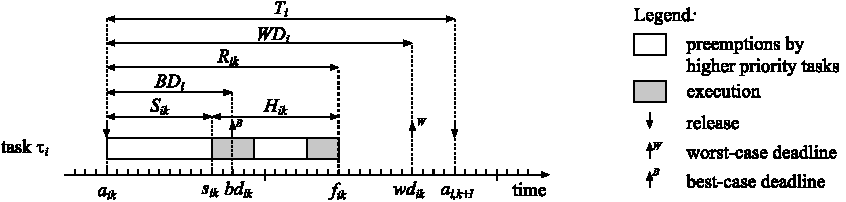
\includegraphics[width=1\linewidth]{fig/task_model_2}
	\caption{Basic model for a periodic task $\tau_i$.}
	\label{fig:taskmodel}
\end{figure*}

Each task $\tau_i$ generates an infinite sequence of jobs $\iota_{ik}$ with $k\in \mathbb{Z}$. In addition, each task is characterized by a \textit{period} $T_i \in \mathbb{R^{+}}$, a \textit{worst-case computation time} $\wc_i \in \mathbb{R^{+}}$, a \textit{best-case computation time} $\bc_i \in \mathbb{R^{+}}$, where $\bc_i \leq \wc_i$, a \textit{phasing} $\phi_i \in \mathbb{R}$, a (relative) \textit{worst-case deadline} $\wcd_i \in \mathbb{R^{+}}$, and a (relative) \textit{best-case deadline} $\bd_i \in \mathbb{R^{+}}\cup \{0\}$, where $\bd_i \leq \wcd_i$. We assume arbitrary phasings. Moreover, the set of phasings $\phi_i$ is termed the phasing $\phi$ of the task-set $\mathpzc{T}$. Furthermore, we assume arbitrary deadlines; hence, deadline $\wcd_i$ may be smaller than, equal to, or larger than period $T_i$. In addition, we assume that tasks do not suspend themselves, jobs do not start before the completion of previous jobs of the same task, and the overhead of context switching and task scheduling is ignored.

For FPTS, each task $\tau_i$ has an additional property called \textit{preemption threshold} denoted by $\theta_i$, where $\pi_1 \geq \theta_i \geq \pi_i$. A task $\tau_i$ can be preempted by a higher priority task $\tau_h$ if and only if $\pi_h > \theta_i$. FPPS is a special case of FPTS when $\forall_{1\leq i \leq n}\theta_i = \pi_i$, and FPNS is a special case when $\forall_{1\leq i \leq n}\theta_i = \pi_1$.

It is worth noting that activation jitter is ignored in the real-time scheduling model under study. We aim to first investigate the best-case response times analysis for FPTS for the basic model before refining the model with the notion of activation jitter.

\subsection{Derived notions}
Given the \textit{activation time} $a_{i,k}$ of the $k^{th}$ job of a task $\tau_i$ and its (absolute) \textit{finalization time} $f_{i,k}$, the \textit{response time} $R_{i,k}$ of such a job is defined as the time elapsed between its finalization and activation, i.e. $R_{i,k}=f_{i,k}-a_{i,k}$. The \textit{absolute start time} $s_{i,k}$ is the time at which job $k$ of $\tau_i$ starts its execution. Furthermore, the \textit{relative start time} $S_{i,k}$ is the start time relative to the activation of a job, i.e. $S_{i,k}=s_{i,k}-a_{i,k}$. Finally, we define the \textit{hold time} $H_{i,k}$ as the time elapsed between the start of a job and its completion, this is expressed as $H_{i,k}=f_{i,k}-s_{i,k}$. In general, under this model, it always holds that $R_{i,k}=S_{i,k}+H_{i,k}$. Figure \ref{fig:taskmodel} shows the basic task model with these notions.

The \textit{worst-case response time} $\wr_i$ and the \textit{best-case response time} $\br_i$ of a task $\tau_i$ are defined as the longest and the shortest response times of its jobs respectively, i.e.
\begin{align}
	\wr_i \defeq \text{sup}_{\phi,k} R_{i,k}(\phi)\\
	\br_i \defeq \text{inf}_{\phi,k} R_{i,k}(\phi),
\end{align}
where $R_{i,k}(\phi)$ denotes a dependency of response time $R_{i,k}$ on phasing $\phi$.

We say that a set $\mathpzc{T}$ of $n$ periodic tasks is schedulable if and only if
\begin{align}
	\displaystyle\mathop{\forall}_{1 \leq i \leq n}(\bd_i\leq \br_i \land \wr_i \leq \wcd_i).
\end{align}

Finally, we introduce the notion of level-$i$ active period and best-case utilization. In order to define the notion of level-$i$ active period \cite{BLV09}, we first introduce the notion of pending load. The \textit{pending load} $P_i(t)$ of a task $\tau_i$ is defined as the amount of processing at time $t$ that still needs to be completed for the jobs with a priority higher than or equal to task $\tau_i$ that are activated before time $t$. A level-$i$ active period is then defined as the interval $[t_s,t_e)$ such that $P_i(t_s)=0$, $P_i(t_e)=0$, and $P_i(t)>0$ for all $t \in (t_s,t_e)$.

We define the best-case utilization $\bu^{\mathpzc{T}}$ as the best-case fraction of the  processor time spent on the execution of $\mathpzc{T}$, i.e.

%A common term used in the response-time analysis of scheduling policies is the notion of level-$i$ active period \cite{BLV09}. To define this notion, we first introduce the notion of pending load. The \textit{pending load} $P_i(t)$ of a task $\tau_i$ is defined as the amount of processing at time $t$ that still needs to be completed for the jobs with a priority higher than or equal to task $\tau_i$ that are activated before time $t$. A level-$i$ active period is then defined as the interval $[t_s,t_e)$ such that $P_i(t_s)=0$, $P_i(t_e)=0$, and $P_i(t)>0$ for all $t \in (t_s,t_e)$.
%
%Finally, we define the best-case utilization $\bu^{\mathpzc{T}}$ as the best-case fraction of the  processor time spent on the execution of $\mathpzc{T}$, i.e.
\begin{align}
\bu^{\mathpzc{T}} \defeq \sum_{1\leq i \leq n} \frac{\bc_i}{T_i}.
\end{align} 

\section{Best-case response time for non-preemptive tasks}
Since FPNS is a special case of FPTS when thresholds of tasks are set to the highest priority, we first investigate the best-case response time for non-preemptive tasks as an intermediate step towards the best-case analysis for FPTS.

\begin{lemma}
	\textit{Let $\tau_i$ be a non-preemptive task, i.e. $\theta_i = \pi_1$, and let $\bu^{\mathpzc{T}}<1$ or $\bu^{\mathpzc{T}}=1$ and the lcm of the periods exists. The \textit{best-case response time} of $\tau_i$ is always equal to its \textit{best-case computation time}, i.e. $\br_i = \bc_i$.}
\end{lemma}

\begin{proof}
	Given a task-set $\mathpzc{T}$ and a non-preemptive task $\tau_i \in \mathpzc{T}$, assume that all jobs of $\tau_i$ have a computation time equal to $\bc_i$. Since $\tau_i$ is non-preemptive, the hold time of all its jobs is simply equal to $\bc_i$. Recall that the response time of a job $k$ of $\tau_i$ is given by $R_{i,k}=S_{i,k}+H_{i,k}$. Therefore, in order to prove the lemma, it is sufficient to show that it is always possible to schedule task $\tau_i$ in such a way that the relative start time of a job $k$ of $\tau_i$ is zero, i.e. $S_{i,k}=0$. We divide this proof in two cases:
	
	\{\textit{Case $\bu^{\mathpzc{T}} < 1$}\}. Given an arbitrary schedule for $\mathpzc{T}$, let $[t_s,t_e)$ with $t_e > t_s$ be an idle interval in such a schedule, where an idle interval is a time interval in which there is no pending load. Note that it is always possible to find an idle interval because $\bu^{\mathpzc{T}} < 1$. Furthermore, let $\iota_{i,k}$  be the first job of $\tau_i$ activated at or after time $t_e$, i.e. $t_e \leq a_{i,k}$. We now show that, by pushing the activation of $\iota_{i,k}$ to occur in the interval $[t_s,t_e)$, the relative start time of $\iota_{i,k}$ becomes zero.
	
	First observe that there is no other job of $\tau_i$ between the idle interval $[t_s,t_e)$ and $\iota_{i,k}$. Hence, after pushing the activations of $\tau_i$ till $a_{i,k}$ occurs in $[t_s,t_e)$, job $\iota_{i,k}$ does not experience blocking by a previous job. Furthermore, since $[t_s,t_e)$ was originally idle, job $\iota_{i,k}$ can start upon activation, leading to $S_{i,k} = 0$.
	
	\{\textit{Case $\bu^{\mathpzc{T}} = 1$ and the lcm of the periods exists}\}. In
	order to prove this case, first recall that the hyperperiod is defined as the length of the shortest time interval in which the schedule repeats itself after an initial start-up. For a set of periodic tasks, Leung and Merrill proved in \cite{LM80} that the hyperperiod $H$ can be calculated as the least common multiple of the periods, i.e. $H=lcm(T_1,...,T_n)$ for $n$ periodic tasks. 
	
	Let $n_i = H/T_i$ be the number of jobs of $\tau_i$ in every hyperperiod and assume that no job of $\tau_i$ starts upon activation. Hence, for each interval $[a_{i,k^{\prime}},s_{i,k^{\prime}})$ with $1 \leq k^{\prime} \leq n_i$, there are only higher priority tasks of $\tau_i$ and/or at most one blocking lower priority task executing within such an interval. As an example of this situation, consider the timeline depicted in Figure \ref{fig:fpns1} for task-set $\mathpzc{T}_{\ref{tab:taskset1}}$ described in Table \ref{tab:taskset1}. As can be seen, no job of $\tau_2$ can start upon activation.
	
%	 Furthermore, let $\iota_{i,1}$ and $\iota_{i,n_i}$ be the first and last job of $\tau_i$ respectively in an hyperperiod.

	\begin{table}[h]
		\center
		\caption{Task characteristics of $\mathpzc{T}_{\ref{tab:taskset1}}$.}
		\label{tab:taskset1}
		\begin{tabular}{c | c c c c c}
			\hline 
			task & $T_i$ & $\wcd_i$ & $C_i$ & $\pi_i$ & $\theta_i$  \\ 
			\hline 
			$\tau_1$& 4 & 4 & 2  & 2 & 2\\ 
			$\tau_2$& 6 & 6 & 3  & 1 & 2\\ 
			\hline 
		\end{tabular}
		\small
		\item The hyperperiod is $H=12$ and $\bu^{\mathpzc{T_{\ref{tab:taskset1}}}}=1$.
	\end{table}
	
	\begin{figure}[h]
		\centering
		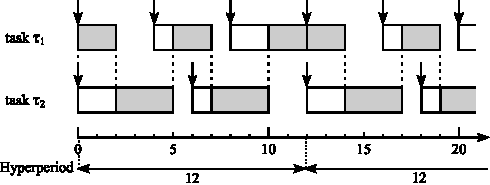
\includegraphics[width=1\linewidth]{fig/fpns1}
		\caption{A timeline for $\mathpzc{T}_{\ref{tab:taskset1}}$. The activations of the tasks are repeated in every interval with length $H=12$.}
		\label{fig:fpns1}
	\end{figure}
	
	Now let $\iota_{i,k}$ be the job of $\tau_i$ with the shortest relative start time among all jobs of $\tau_i$ in an hyperperiod. Since no job of $\tau_i$ starts upon activation, we can push the activation of all jobs of $\tau_i$ to a later moment in time, without modifying the schedule, till job $\iota_{i,k}$ starts upon activation. After pushing the activations of $\tau_i$, it holds that $S_{i,k}=0$ therefore concluding the proof. Figure \ref{fig:fpns2} shows an example where the schedule shown in Figure \ref{fig:fpns1} is preserved after pushing the activations of $\tau_2$ till its second job starts upon activation.	
%	
%		Now let $\iota_{i,k}$ be the job of $\tau_i$ with the shortest relative start time among all jobs of $\tau_i$ in an hyperperiod. Since no job of $\tau_i$ starts upon activation and $\iota_{i,k}$ is the job with the shortest start time, we can push
\end{proof}

\begin{figure}[h]
	\centering
	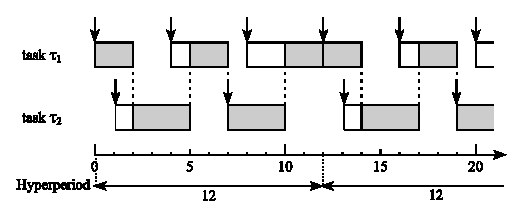
\includegraphics[width=1\linewidth]{fig/fpns2}
	\caption{A timeline for $\mathpzc{T}_{\ref{tab:taskset1}}$. After pushing the activations of $\tau_2$, the second job can immediately start.}
	\label{fig:fpns2}
\end{figure}

\section{Towards best-case analysis for FPTS}

In this section, we illustrate by means of an example that the best-case response time analysis for FPTS is most likely not a trivial extension of the existing best-case analysis for FPPS.
%
\subsection{Recap of optimal instant for FPPS}
An optimal instant is defined as the (hypothetical) instant that leads to the best-case response time of a task. For FPPS, the notion of optimal instant is the following \cite{BLM13}:
\begin{theorem}
	An optimal instant of a task $\tau_i$ under FPPS and arbitrary deadlines occurs when the completion of a job of task $\tau_i$ coincides with the simultaneous activation of all its higher priority tasks. 
\end{theorem}

It is worth noting that, for FPPS, the job experiencing the optimal instant is the job that assumes the best-case response time. Furthermore, such a job is also the last job in its level-$i$ active period.
%
%For FPNS, a conjecture of a so called $\Delta$-optimal instant is presented in \cite{BV05}. Based on this conjecture, a lower bound for the best-case response time under FPNS is also derived.
%
%\begin{conjecture}
%	A $\Delta$-optimal instant of a task $\tau_i$ under FPNS occurs when a job of $\tau_i$ starts a sufficintly small amount of time $\Delta > 0$ before the simultaneous activation of all its higher priority tasks.
%\end{conjecture} 

\subsection{An introductory example}
From Lemma 1, we can conclude that the best-case response time of a non-preemptive task  is independent of higher priority tasks. Based on this, it could be tentative to think that, given a task $\tau_i$ scheduled under FPTS, the best-case response time of $\tau_i$ would be independent of all its higher priority tasks that cannot preempt it, i.e. the tasks in $\{\tau_h | \theta_i \geq \pi_h > \pi_i\}$. However, this is not the case for FPTS as we show in the following example.

\begin{figure*}
	\centering
	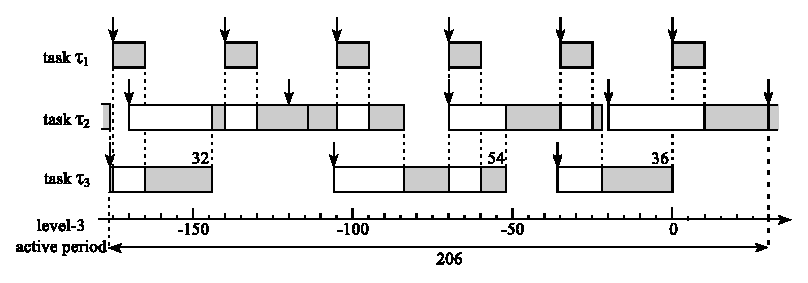
\includegraphics[width=0.66\linewidth]{fig/fpps_fact1_3}
	\caption{A timeline for $\mathpzc{T}_{\ref{tab:taskset2}}$ depicting a level-3 active period. The best-case response time of $\tau_3$ is assumed by the first job in the level-3 active period.}
	\label{fig:fpps_fact1}
\end{figure*}

% The activation of the highest priority task $\tau_1$ coincides with the completion of job $\iota_{3,1}$ of task $\tau_3$ at time $t=0$. Furthermore, task $\tau_2$ is activated a small time $\Delta > 0$ after the start time of $\iota_{3,1}$.

%Based on the notion of optimal instant for FPPS, it could be tentative to think that an optimal instant for FPTS may occur when the completion of a job of a task $\tau_i$ coincides with the simultaneous activation of all higher priority tasks that can preempt $\tau_i$. These are the tasks in $\{\tau_h | \pi_h > \theta_i \}$. In this section, we introduce an example that refutes this intuition of optimal instant for FPTS.

%under FPTS, the best-case response time of a task $\tau_i$ could be found in a job which completion coincides with the simultaneous activation of all higher priority tasks that can preempt $\tau_i$. These are the tasks in $\{\tau_h | \pi_h > \theta_i \}$. In this section, we introduce an example that refutes this intuition.

\begin{table}[h]
	\center
	\caption{Task characteristics of $\mathpzc{T}_{\ref{tab:taskset2}}$.}
	\label{tab:taskset2}
	\begin{tabular}{c | c c c c c | c c}
		\hline 
		task & $T_i$ & $\wcd_i$ & $\wc_i=\bc_i$ & $\pi_i$ & $\theta_i$ &  $\wr_i$ & $\br_i$\\ 
		\hline 
		$\tau_1$& 35 & 20 & 10 & 3 & 3 &  10 & 10\\ 
		$\tau_2$& 50 & 65 & 20 & 2 & 2 &  62 & 20\\ 
		$\tau_3$& 70 & 70 & 22 & 1 & 2 &  66 & 32\\
		\hline 
	\end{tabular}
	\small
	\item The \textit{least common multiple} of the periods is 350 and $\bu^{\mathpzc{T_{\ref{tab:taskset2}}}}=1$.
\end{table}

Consider the set $\mathpzc{T}_{\ref{tab:taskset2}}$ of three tasks with characteristics as described in Table \ref{tab:taskset2}. The best-case response time values in this table were found using brute force. This is, by considering the phasings $\phi_1 \in [0,35)$ and $\phi_2 \in [0,50)$ with a granularity of one time unit in the simulations, while fixing the phasing of $\tau_3$ to $\phi_3 = 0$. Furthermore, note that task $\tau_1$ can preempt task $\tau_3$ because $\pi_1 > \theta_3$. On the other hand, task $\tau_2$ cannot preempt task $\tau_3$ because $\pi_2 = \theta_3$. 


Figure \ref{fig:fpps_fact1} shows a timeline for task-set $\mathpzc{T}_{\ref{tab:taskset2}}$ where the best-case response time of task $\tau_3$ is assumed by the first job in the level-3 active period. As can be seen, this best-case response time is assumed when $\tau_3$ experiences one preemption by task $\tau_1$; hence, resulting in $\br_3 = 32$. However, when ignoring task $\tau_2$ from task-set $\mathpzc{T}_{\ref{tab:taskset2}}$, the best-case response time of task $\tau_3$ is reduced to $\br_3 = 22$. Based on this observation, we conclude that, in general, the best-case response time of a task $\tau_i$ is not independent of the higher priority tasks that cannot preempt $\tau_i$. Therefore, we formulate the following fact.

\begin{fact}
	In FPTS, the best-case response time of a preemptive task $\tau_i$, i.e. $\pi_1 > \theta_i$, can also be affected by a higher priority task that cannot preempt $\tau_i$.
\end{fact}

From Figure \ref{fig:fpps_fact1}, we can also observe that an activation of $\tau_1$ coincides with the completion of a job of $\tau_3$ at time $t=0$. This is similar to the notion of optimal instant for FPPS. However, the best-case response time is not assumed by such a job ending at time $t=0$. Therefore, we have a first witness of dissimilarity between the best-case response time analysis for FPPS and FPTS.

\begin{fact}
	In FPTS, a job k of task $\tau_i$ does not necessarily assume the best-case response time when the activation of all higher priority tasks that can preempt task $\tau_i$ coincides with the completion of job k.
\end{fact}

Furthermore, an important property in the best-case analysis for FPPS and arbitrary deadlines is that the last job in a level-$i$ active period always experiences the shortest response time of all jobs in that level-$i$ active period. This property was highlighted in \cite{BLM13} as a witness of non-duality between best-case and worst-case analysis. This property clearly does not hold for FPTS as shown in Figure \ref{fig:fpps_fact1}. As can be seen, the first job in the level-3 active period is the one with the shortest response time. Based on this, we introduce the following fact as second witness of dissimilarity between the best-case behavior of FPPS and FPTS.

\begin{fact}
	In FPTS, the shortest response time of a task $\tau_i$ in a level-$i$ active period is not necessarily assumed by the last job in that level-$i$ active period.
\end{fact}


%Therefore, we introduce the following fact.

%The worst-case response time values in Table \ref{tab:taskset2} were found by applying the worst-case response time analysis for FPTS in \cite{bibid}.


%Figure \ref{fig:fpps_fact1} shows a timeline for task-set $\mathpzc{T}_{\ref{tab:taskset2}}$ with the configuration that we aim to refute for the last job of task $\tau_3$. As can be seen, the completion of this job coincides with an activation of the highest priority task $\tau_1$ at time $t=0$. Note that task $\tau_1$ can preempt task $\tau_3$ because $\pi_1 > \theta_3$. On the other hand, task $\tau_2$ cannot preempt task $\tau_3$ because $\pi_2 = \theta_3$. For the latter reason, the activation of task $\tau_2$ is set to a sufficiently small amount of time $\Delta>0$ after the start time of the last job of task $\tau_3$, therefore, allowing more time before $t=0$ for the execution of task $\tau_3$. This is in accordance with the notion of $\Delta$-optimal instant.

%to an earlier moment in time in Figure \ref{fig:fpps_fact1}, allowing more time before $t=0$ for the execution of task $\tau_3$.

%As can be seen from Figure \ref{fig:fpps_fact1}, the last job of task $\tau_3$ that is experiencing the new optimal instant has a response time of $R_{3,1}=36$. However, the best-case response time of task $\tau_3$ is $\br_3 = 32$, and it is assumed by the job activated at time $t=-176$. Note also that the response time of the job experiencing the optimal instant cannot be reduced by pushing the activations of task $\tau_3$ because the job activated at time $t=-176$ already can start upon activation. Hence, pushing the activations of task $\tau_3$ to a later moment in time would modify the schedule.


%From Figure \ref{fig:fpps_fact1}, we can also observe that, in order to calculate the response time of job $\iota_{3,1}$, we have to look at previous jobs in the level-3 active period to see whether they induce some delay in the start time of $\iota_{3,1}$. This is similar to the best-case response time analysis for FPPS in \cite{BLM13}. An important property for this analysis, however, is that under FPPS the last job in a level-$i$ active period always experiences the shortest response time of all jobs in that level-$i$ active period. This property clearly does not hold for FPTS as shown in Figure \ref{fig:fpps_fact1}. As can be seen, the first job in the level-3 active period is the one with the shortest response time. Therefore, we introduce the following fact.

\section{Conclusion}
In this paper, we proved that the best-case response time of a non-preemptive task is equal to its best-case computation time when scheduled under FPTS or FPNS. In addition, we showed some witnesses of dissimilarity between the best-case behaviors of FPPS and FPTS. We therefore conclude that the best-case analysis for FPTS is most likely not a trivial extension of the current analysis for FPPS. An exact best-case response time analysis for FPTS is currently under study.


%\ifCLASSOPTIONcompsoc
%  % The Computer Society usually uses the plural form
%  \section*{Acknowledgments}
%\else
%  % regular IEEE prefers the singular form
%  \section*{Acknowledgment}
%\fi
%
%
%The authors would like to thank...
%
%



% trigger a \newpage just before the given reference
% number - used to balance the columns on the last page
% adjust value as needed - may need to be readjusted if
% the document is modified later
%\IEEEtriggeratref{8}
% The "triggered" command can be changed if desired:
%\IEEEtriggercmd{\enlargethispage{-5in}}

% references section

% can use a bibliography generated by BibTeX as a .bbl file
% BibTeX documentation can be easily obtained at:
% http://mirror.ctan.org/biblio/bibtex/contrib/doc/
% The IEEEtran BibTeX style support page is at:
% http://www.michaelshell.org/tex/ieeetran/bibtex/
%\bibliographystyle{IEEEtran}
% argument is your BibTeX string definitions and bibliography database(s)
%\bibliography{IEEEabrv,../bib/paper}
%
% <OR> manually copy in the resultant .bbl file
% set second argument of \begin to the number of references
% (used to reserve space for the reference number labels box)
\begin{thebibliography}{1}

\bibitem{TX}	
Express Logic Inc. ThreadX Technical Features, v5.1. [Online].
Available: http://rtos.com/products/threadx, June 2010.

\bibitem{AUT10}
{AUTOSAR} -- \textit{Specification of Operating System}, {Release}~4.1.
2010.
[Online], Available: http://www.autosar.org/

%\bibitem{B11}
%S. Bunzel.
%\textit{AUTOSAR - the standardized software architecture}.
%Informatik-Spektrum, vol. 34, no. 1, pp. 79-83, 2011.

\bibitem{OSEK05}
OSEK group,
{OSEK/VDX} \textit{Operating System}.
February 2005.
[Online], Available: http://portal.osek-vdx.org/files/pdf/specs/os223.pdf.

\bibitem{WS99}
Y. Wang and M. Saksena.
\textit{Scheduling fixed-priority tasks with preemption threshold}.
In Proc. 6th International Conf. Real-Time Computing Systems and Applications. (RTCSA), pp. 328-335, Dec. 1999.

\bibitem{R02}
J. Regehr.
\textit{Scheduling tasks with mixed preemption relations for robustness to timing faults}.
In Proc. 23rd IEEE Real-Time Systems Symposium (RTSS),
pp. 315-326,
December 2002.

\bibitem{KRL05}
U. Keskin, R.J. Bril, and J.J. Lukkien.
\textit{Exact response-time analysis for fixed-priority preemption-threshold scheduling.} 
In IEEE Conf. Emerging Technologies and Factory Automation (ETFA), pp. 1–4, Sep. 2010.

\bibitem{RS02}
O. Redell and M. Sanfridson.
\textit{Exact best-case response time analysis of fixed priority scheduled tasks}.
In Proc. 14th Euromicro Conference on Real-Time Systems (ECRTS),
pp. 165-172, June 2002.

\bibitem{BLM13}
R.J. Bril, J.J. Lukkien, and R.H. Mak.
\textit{Best-case response times and jitter analysis of real-time tasks with arbitrary deadlines.}
In Proc. 21st International Conference on Real-Time Networks and Systems (RTNS), ACM, pp. 193-202, October 2013.

\bibitem{DBBL07}
R.I. Davis, A. Burns, R.J. Bril, J.J. Lukkien.
\textit{Controller Area Network (CAN) schedulability analysis: refuted, revisited and revised.}
In Real-Time Systems journal, 
35(3):239-272, April 2007.

\bibitem{BLV09}
R.J. Bril, J.J. Lukkien, W.F.J. Verhaegh.
\textit{Worst-case response time analysis of real-time tasks under fixed-priority scheduling with deferred preemption}.
In Real-Time Systems journal, 42(1-3):63-119, Aug. 2009.

\bibitem{BV05}
R.J. Bril, W.F.J. Verhaegh.
\textit{Towards best-case response times of real-time tasks under fixed-priority scheduling with deferred preemption.}
In Proc. Work-in-Progress (WiP) session of the 17th Euromicro Conf. on Real-Time Systems (ECRTS), pp. 17-20, July 2005.

\bibitem{LM80}
J.~Leung, R.~Merrill. \textit{A note on the preemptive scheduling
	of periodic, real-time tasks}. 
Information Processing Letters,
11(3):115-118, November 1980.

\end{thebibliography}




% that's all folks
\end{document}


